\chapter{Matrices}\label{app:matrices}
This appendix aims to provide some fundamental knowledge on matrices and linear algebra used throughout this thesis. 

A matrix is a rectangular array with numerical elements and its dimensions are denoted using ``$row \times column$''. A $3\times 5$ matrix, for example, thus has $3$ rows and $5$ columns (see Figure \ref{fig:matrixA}). Along those lines, a \textit{row vector} is a matrix with $1$ row and more than $1$ column and a \textit{column vector} is a matrix with $1$ column and more than $1$ row.

In this document, matrices and vectors are written using bold symbols. %\SWcomment[Many notations exist, blabla $\bar a$ $\vec a$] 
A matrix is denoted by a capital letter -- such as $\A$ -- whereas vectors are decapitalised -- such as $\u$. An element in a matrix is denoted with a non-bold, decapitalised variable, where the subscripts indicate the indices of the row and column. For example, the element in the 2\textsuperscript{nd} row and the 4\th column of a matrix $\A$ is denoted as $a_{24}$. An element in a vector only has one subscript, regardless of whether it is a row or a column vector.

\section{Operations}
Multiplying and dividing a matrix by a scalar (a single number) is valid and happens on an element-by-element basis. For a $2\times 2$ matrix $\A$ and scalar $p$ the following operations hold
\begin{equation*}
        p \A = \A p = \begin{bmatrix}
        p\cdot a_{11}& p\cdot a_{12}\\
        p\cdot a_{21} & p\cdot a_{22}
    \end{bmatrix}, \qaq \A / p= \begin{bmatrix}
            a_{11}/p& a_{12}/p\\
            a_{21}/p & a_{22}/p
    \end{bmatrix}.
\end{equation*}
Notice that although a matrix can be divided by a scalar, a scalar can not necessarily be divided by a matrix. See Section \ref{sec:inverse} for more information.

\subsubsection{Matrix transpose}
A matrix or vector can be \textit{transposed}, which is indicated by the $T$ operator. Transposing a matrix $\A$ is denoted by $\A^T$. This means that the elements in the $i$\th row and the $j$\th column of the original matrix become the elements in the $j$\th row and the $i$\th column of the transposed matrix. Essentially the row and column indices of the elements inside the matrix get switched according to
\begin{equation}\label{eq:matrixTransposition}
    a_{ij} = a_{ji}.
\end{equation} 
Also see Figure \ref{fig:matrixTransp}. For a row vector, the transpose operation simply changes it to a column vector and vice versa. Another way of seeing a transpose is that all the elements get flipped over the \textit{main diagonal} of the matrix. The main diagonal comprises the elements $a_{ij}$ where $i=j$ and a transpose does not affect the location of these elements. 

\begin{figure}[h]
    \centering
    \subfloat[A $3\times 5$ matrix $\A$.\label{fig:matrixA}]{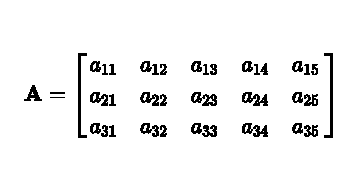
\includegraphics[width=0.45\textwidth]{figures/analysis/matrixA1.pdf}}\hspace{0.03cm}
    \subfloat[A transposed matrix $\A^T$ of size $5\times 3$.\label{fig:matrixAT}]{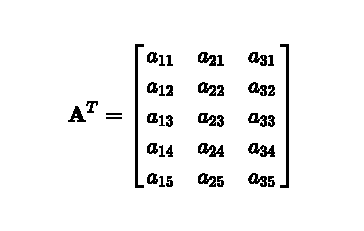
\includegraphics[width=0.45\textwidth]{figures/analysis/matrixAT1.pdf}}
    \caption{A matrix $\A$ and its transpose $\A^T$. The elements get flipped along the main diagonal of the matrix according to Eq. \eqref{eq:matrixTransposition}. \label{fig:matrixTransp}}
\end{figure}

\subsubsection{Matrix multiplication}
Matrix multiplication (this includes matrix-vector multiplication) is different from regular multiplication in that it needs to abide several extra rules. The multiplication of two matrices $\A$ and $\B$ to a resulting matrix $\C$ is defined as
\begin{equation}\label{eq:matrixMult}
    c_{ij} = \sum_{k=1}^K a_{ik} b_{kj},
\end{equation}
where $K$ is both the number columns of matrix $\A$ and the number of rows in matrix $\B$. It thus follows that, in order for a matrix multiplication to be valid, the number of columns of the first matrix needs to be equal to the number of rows in the second matrix. The result will then be a matrix with a number of rows equal to that of the first matrix and a number of columns equal to that of the second matrix. See Figure \ref{fig:matrixVector} for reference.

As an example, consider the $L\times M$ matrix $
\A$ and a $M\times N$ matrix $\B$ with $L\neq N$. The multiplication $\A\B$ is defined as the number of columns of matrix $\A$ ($M$) is equal to the number of rows of matrix $\B$ (also $M$). The result, $\C$, is a $L \times N$ matrix. The multiplication $\B\A$ is undefined as the number of columns of the first matrix does not match the number of rows in the second matrix. A valid multiplication of two matrices written in their dimensions is
\begin{equation}
    \overbrace{(L\times M)}^{\A}\cdot \overbrace{(M\times N)}^{\B} = \overbrace{(L
    \times N)}^{\C}.
\end{equation}

\begin{figure}[h]
    \centering
    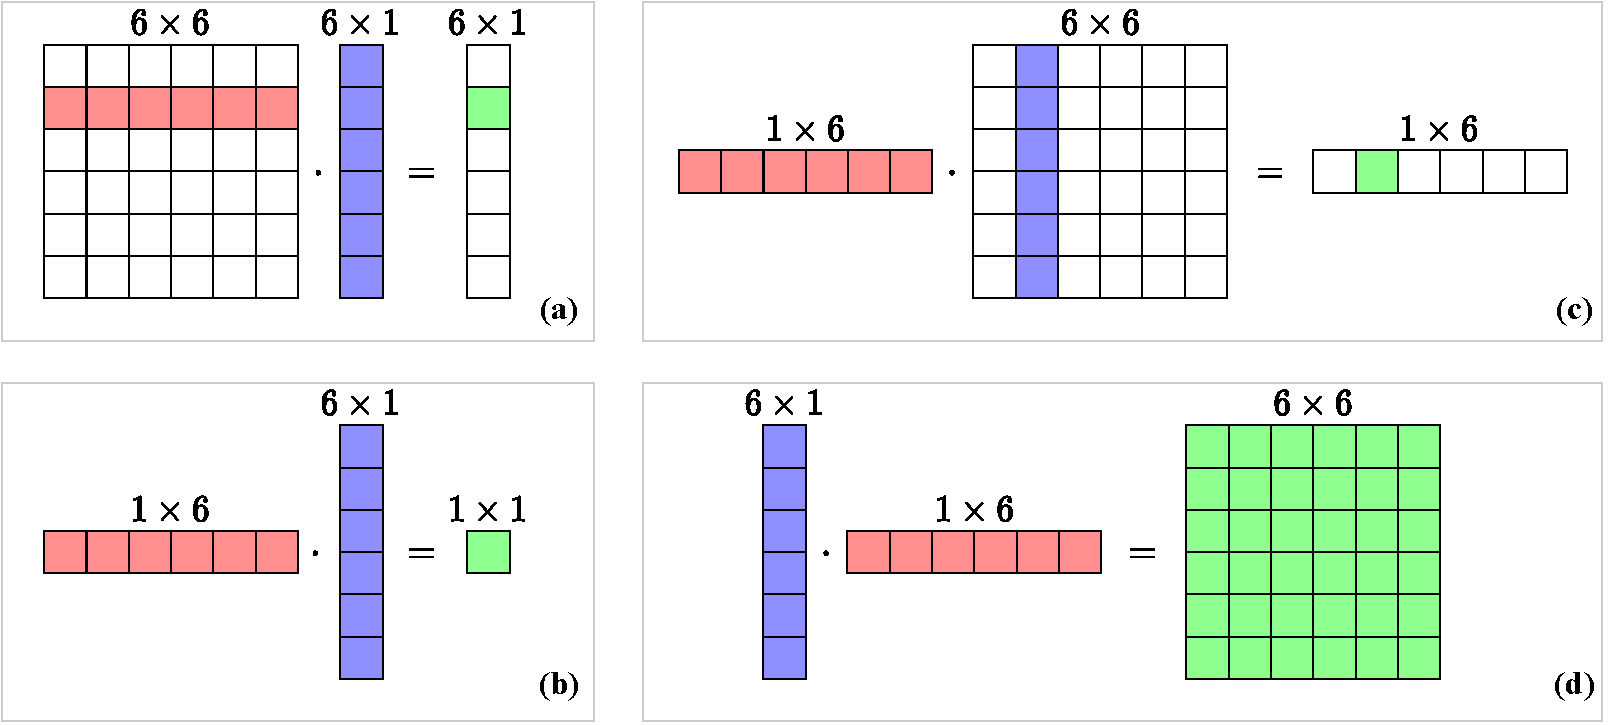
\includegraphics[width=\textwidth]{figures/analysis/matrixVector.pdf}
    \caption{Visualisation of valid matrix multiplications (see Eq. \eqref{eq:matrixMult}). The ``inner'' dimensions (columns of the left matrix and rows of the right) must match and result in a matrix with a size of ``outer'' dimensions (rows of the left matrix and columns of the right). \label{fig:matrixVector}}
\end{figure}

\section{Matrix inverse}\label{sec:inverse}
If a matrix has the same number of rows as columns, it is called a \textit{square matrix}. Square matrices have special properties, one of which is that it (usually) can be \textit{inverted}. A square matrix $\A$ is invertible if there exists a matrix $\B$ such that
\begin{equation}
    \A \B = \B \A = \I. 
\end{equation}
This matrix $\B$ is then called the \textit{inverse} of $\A$ and can be written as $\A^{-1}$. Not all square matrices have an inverse, in which case it is called \textit{singular}. Rather than going through manually inverting a matrix, or determining whether it is singular, the following function in \texttt{MATLAB} will provide the inverse of a matrix \texttt{A}:
\begin{center}
    \texttt{A\_inverted = inv(A);}
\end{center}

The inverse of a \textit{diagonal matrix} (a matrix with non-zero elements on its main diagonal and the rest zeros) is obtained by replacing the diagonal elements by their reciprocal. So for a diagonal $3\times 3$ matrix, the following holds:
\begin{equation*}
    \xbracketMatrixstack{
        a_{11} & 0 & 0\\
        0 & a_{12} & 0\\
        0 & 0 & a_{33}
    }^{-1} =\quad 
    \xbracketMatrixstack{
        \frac{1}{a_{11}} & 0 & 0\\
        0 & \frac{1}{a_{12}} & 0\\
        0 & 0 & \frac{1}{a_{33}}
    }.
\end{equation*}

\section{Systems of linear equations}\label{sec:linearEquations}
Matrices can be conveniently used to solve \textit{systems of linear equations}, a set of linear equations containing the same set of variables. 

For example, take the system of linear equations
\begin{align*}
    x + z &= 6,\\
    z - 3y &= 7,\\
    2x + y + 3z &= 15,
\end{align*}
with independent variables $x$, $y$ and $z$. The goal is to find a solution for these variables that satisfy all three equations. This system could be solved by hand using algebraic methods, but alternatively, the system can be written in matrix form:
\begin{equation}
    \A \u = \w.
\end{equation}
Here, column vector $\u$ contains the independent variables $x$, $y$, and $z$, matrix $\A$ contains the coefficients multiplied onto these variables and $\w$ contains the right-hand side, i.e., the coefficients not multiplied onto any of the variables:
\begin{equation*}
    \underbrace{\xbracketMatrixstack{
        1& 0& 1\\
        0& -3& 1\\
        2& 1& 3}}_{\A}
    \underbrace{\xbracketMatrixstack{
        x\\
        y\\
        z
    }}_{\u} = \underbrace{\xbracketMatrixstack{
        6\\
        7\\
        15
    }}_{\w}
\end{equation*}
This can be solved for $\u$ by taking the inverse of $\A$ (see Section \ref{sec:inverse}) and multiplying this onto $\w$
\begin{equation}
    \u = \A^{-1}\w.
\end{equation}
Generally, if X unknowns are described by X equations, the unknowns can be solved for, by using this method.

Solving a system of linear equations can be implemented in \texttt{MATLAB} by using the code given in Section \ref{sec:inverse} and multiplying this onto a vector \texttt{w}
\begin{center}
    \texttt{u = inv(A) * w;}
\end{center}
or more compactly, by using the `\texttt{\textbackslash}' operator:
\begin{center}
    \texttt{u = A\textbackslash w;}
\end{center}

\section{Eigenvalue problems}\label{sec:eigenValueProblems}
A square matrix $\A$ is characterised by its \textit{eigenvalues} and corresponding \textit{eigenvectors}. In a FDTD context, these are usually associated with the modes of a system, where the eigenvalues relate to the modal frequencies and the eigenvectors to the modal shapes. Section \ref{sec:modalAnalysis} provides more information on this.

To find these characteristic values for a $p\times p$ matrix $\A$, an equation of the following form must be solved 
\begin{equation}
    \A \boldPhi = \lambda \boldPhi.
\end{equation}
This is called is an \textit{eigenvalue problem} and has $p$ solutions (corresponding to the dimensions of $\A$). These are the $p$\th eigenvector $\boldPhi_p$ and the corresponding eigenvalue $\lambda_p$ which is calculated using
\begin{equation}
    \lambda_p = \eig_p(\A),
\end{equation}
where $\eig_p(\cdot)$ denotes the `$p$\th eigenvalue of'. Instead of delving too deep into eigenvalue problems and the process of how to solve them, an easy way to obtain the solutions using \texttt{MATLAB} is provided here:

\begin{center}
    \texttt{[phi, lambda] = eig(A, {\color[HTML]{A100F4}'vector'});}
\end{center}
The $p$\th eigenvector appears in the $p$\th column of $p\times p$ matrix \texttt{phi} and the corresponding eigenvalues are given in a $p \times 1$ column vector \texttt{lambda}. %Note that the outcome is not necessarily sorted! To do this, do 
%
% \begin{center}
%     \begin{tabular}{l}
%     \texttt{[lambda, order] = sort(lambda);}\\
%     \texttt{phi = phi(:, order);}
%     \end{tabular}
% \end{center}
